% -----------------------------------------------
% Template for ISMIR LBD Papers
% 2021 version, based on previous ISMIR templates

% Requirements :
% * 2+n page length maximum
% * 10MB maximum file size
% * Copyright note must appear in the bottom left corner of first page
% * Clearer statement about citing own work in anonymized submission
% (see conference website for additional details)
% -----------------------------------------------

\documentclass{article}


\usepackage[T1]{fontenc} % add special characters (e.g., umlaute)
\usepackage[utf8]{inputenc} % set utf-8 as default input encoding
\usepackage{ismir,amsmath,cite,url}
\usepackage{graphicx}
\usepackage{color}

\def\lbd{}	% Flag to use correct LBD settings in the paper, please do not modify this line

\newcommand{\cd}[1]{{\textcolor{blue}{[CD: #1]}}}
\newcommand{\pl}[1]{\textcolor{red}{[PL: #1]}}
% \newcommand{\cd}[1]{}
% \newcommand{\pl}[1]{}

\usepackage{lineno}
\linenumbers

% Title. Please use IEEE-compliant title case when specifying the title here,
% as it has implications for the copyright notice
% ------
\title{
%Transcribing multitrack music audio into lead sheets
Sheet Sage: Lead Sheets from Music Audio
}

% Note: Please do NOT use \thanks or a \footnote in any of the author markup

% Single address
% To use with only one author or several with the same address
% ---------------
%\oneauthor
% {Names should be omitted for double-blind reviewing}
% {Affiliations should be omitted for double-blind reviewing}

% Two addresses
% --------------
\twoauthors
 {Chris Donahue} {Stanford}
 {Percy Liang} {Stanford}

% Three addresses
% --------------
% \threeauthors
%   {First Author} {Affiliation1 \\ {\tt author1@ismir.edu}}
%   {Second Author} {\bf Retain these fake authors in\\\bf submission to preserve the formatting}
%   {Third Author} {Affiliation3 \\ {\tt author3@ismir.edu}}

% Four or more addresses
% OR alternative format for large number of co-authors
% ------------
%\multauthor
%{First author$^1$ \hspace{1cm} Second author$^1$ \hspace{1cm} Third author$^2$} { \bfseries{Fourth author$^3$ \hspace{1cm} Fifth author$^2$ \hspace{1cm} Sixth author$^1$}\\
%  $^1$ Department of Computer Science, University , Country\\
%$^2$ International Laboratories, City, Country\\
%$^3$  Company, Address\\
%{\tt\small CorrespondenceAuthor@ismir.edu, PossibleOtherAuthor@ismir.edu}
%}

% For the author list in the Creative Common license and PDF metadata, please enter author names. 
% Please abbreviate the first names of authors and add 'and' between the second to last and last authors.
\def\authorname{C. Donahue and P. Liang}

% Optional: To use hyperref, uncomment the following.
\usepackage[bookmarks=false,pdfauthor={\authorname},pdfsubject={\papersubject},hidelinks]{hyperref}
% Mind the bookmarks=false option; bookmarks are incompatible with ismir.sty.

\usepackage{cleveref}
\usepackage{booktabs}

\sloppy % please retain sloppy command for improved formatting

\begin{document}


\maketitle

\begin{abstract}

We present Sheet Sage, 
a system designed to transcribe Western multitrack music into lead sheets: human-readable scores which indicate melody and harmony. 
%\footnote{For music with vocals, lead sheets usually also include lyrics. Here we focus just on transcribing the melody and harmony.} 
The potential use cases for reliable lead sheet transcription are broad and include 
music performance, 
education, 
interaction, 
informatics, 
and generation. 
However, the task is challenging because it involves many subtasks: 
beat tracking, 
key detection, 
chord recognition,
and melody transcription. 
A major obstacle is melody transcription which, 
while arguably simpler for humans than chord recognition, 
remains a challenging task for MIR. 
Here we leverage recent advancements in audio pre-training to break new ground on this task, 
resulting in a system which can reliably detect and transcribe the melody in multitrack recordings. 
By combining this new melody transcription approach with existing strategies for other subtasks, 
Sheet Sage can transcribe recordings into score representations which echo the musical understanding of human experts.\footnote{Examples: \url{http://chrisdonahue.com/sheetsage-lbd}\label{footnote:examples}}
\end{abstract}

\section{Introduction}\label{sec:introduction}

In the Western music canon, 
a musical composition can often be characterized by its melody and harmony. 
% This information can be depicted on a lead sheet---a musical score which contains the melody as notes on a staff and the harmony as chord names. 
% When interpreted by a musician, 
% a lead sheet can be used to perform recognizable renditions of existing pieces.
When engraved as a \emph{lead sheet}---a musical score containing the melody as notes on a staff and the harmony as chord names---melody and harmony can be readily interpreted by musicians, enabling recognizable performances of existing pieces. 
Hence, for some music, a lead sheet represents the essence of its underlying composition.

A system which reliably transcribes multitrack recordings into lead sheets could potentially enrich human music practice by
decreasing the effort required for performing existing pieces, 
which in turn might also increase engagement in music education through curricula tailored to student preferences. 
Moreover, such a system could act as a preprocessing component for MIR pipelines to help facilitate 
interaction~\cite{jenson2016so}, 
informatics~\cite{bainbridge1999towards}, 
retrieval~\cite{ghias1995query}, 
source separation~\cite{ewert2014score}, 
and generation~\cite{hawthorne2019enabling}. 
Despite the numerous potential benefits, 
to the best of our knowledge such a system does not currently exist, 
and building one is challenging as it requires the combination of many individually-difficult MIR tasks: 
beat tracking, 
key detection, 
chord recognition, 
and melody transcription.

Among these tasks, 
\emph{melody transcription}---defined here as converting multitrack audio to a time-aligned, monophonic sequence of equal-tempered notes constituting its melody---is perhaps the furthest from a reliable solution. 
A closely-related problem that has received considerable attention in MIR is \emph{melody extraction}~\cite{goto2000robust}, 
which involves estimating the time-varying fundamental frequency trajectory of the melody in multitrack audio (see~\cite{salamon2014melody} for a comprehensive review). 
While melody extraction is useful for several downstream tasks and is more inclusive of music which does not use equal temperament, 
its outputs cannot be readily converted into familiar music formats like MIDI or scores. 
It is possible to segment the outputs of melody extraction into notes~\cite{nishikimi2016musical}, 
however it stands to reason that the audio contains information about note boundaries that fundamental frequency trajectories lack.
%directly transcribing audio could sidestep the pitfalls of pipeline-based approaches. 
% While melody transcription is possible by segmenting the outputs of melody extraction into notes~\cite{nishikimi2016musical}, 
% it stands to reason that transcribing the melody from audio could outperform pipeline-based approaches.

\begin{figure*}
    \centering
    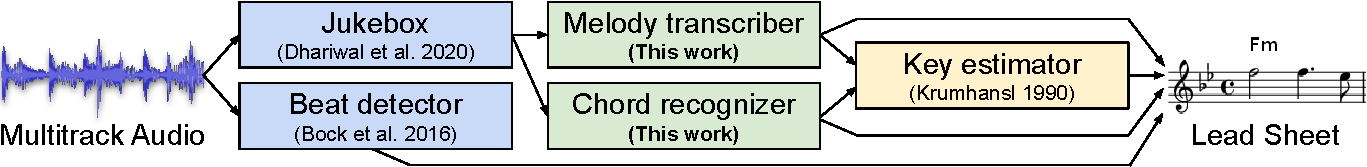
\includegraphics[width=\linewidth]{figs/one.pdf}
    \caption{Inference procedure for Sheet Sage, our proposed system which transcribes multitrack audio into lead sheets (scores which depict melody as notes and harmony as chord names). The blue, green, and yellow boxes respectively take audio, features, and symbolic music data as input. Green boxes are modules that we built as part of this work---both are Transformers~\cite{vaswani2017attention} trained on their respective tasks using audio features from Jukebox~\cite{dhariwal2020jukebox} and data from Hooktheory~\cite{hooktheory}.}
    \label{fig:one}
\end{figure*}

In this work, we break new ground on melody transcription by combining advancements in audio pre-training with a large collection of labeled data for this task. 
Specifically, we collect and align around $50$ hours of paired audio segments and human-transcribed melodies from Hooktheory~\cite{hooktheory}. 
To model this dataset effectively, 
we leverage audio representations from Jukebox~\cite{dhariwal2020jukebox}, 
a generative model pre-trained on one million multitrack recordings. 
These representations were recently shown to be powerful features for several MIR tasks~\cite{castellon2021calm}, 
and here we demonstrate that they are also useful for the task of melody transcription---all else equal, a Transformer~\cite{vaswani2017attention} trained on top of these audio representations achieves
% 0.743 vs 0.587
$27\%$ 
better performance on melody transcription 
than the same architecture trained using traditional spectrogram features.

To complete \emph{Sheet Sage}, 
our lead sheet transcription system, 
we additionally train a chord recognition model using Jukebox representations and data from Hooktheory.
Together, these two models give us estimated timestamps for melody note onsets and chord changes, i.e., a MIDI-like representation. 
Engraving this information as a lead sheet requires additional information: key signature and metrical structure. 
We estimate the former using the Krumhansl-Schmuckler algorithm~\cite{krumhansl1990cognitive,temperley1999key}, which takes the estimated melody and chord information as input. 
For the latter, we use \texttt{madmom}~\cite{bock2016madmom,bock2016joint} to estimate timestamps of beats and downbeats, 
which we then use to quantize the estimated melody and chord transcription to the nearest sixteenth note. 
Finally, we engrave a lead sheet using Lilypond~\cite{nienhuys2003lilypond}. 
See~\Cref{fig:one} for an overview of our system.

\section{Melody Transcription Evaluation}

\begin{figure}[t]
    \centering
    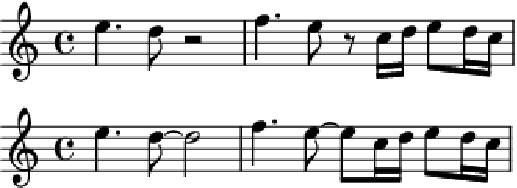
\includegraphics[width=0.95\linewidth]{figs/heuristic_offsets.pdf}
    \caption{
The same note onsets engraved with ground truth~(top) vs. heuristic~(bottom) offsets. 
We argue that 
onset prediction suffices for melody transcription.
%Compared to predicting onsets, we argue that predicting offsets is of secondary importance for human-readable melody transcription.
    }
    \label{fig:heuristic_offsets}
\end{figure}

Services like Chordify~\cite{de2014chordify} already demonstrate that it is possible to estimate all of the information needed for engraving lead sheets besides melody. 
Hence, we focus on melody transcription for our evaluation of Sheet Sage. 
To the best of our knowledge, 
Paiva~et~al.~\cite{paiva2005detection} were the first to investigate melody transcription (rather than extraction). 
The earliest work for which we could find code or audio examples was that of Ryyn{\"a}nen and Klapuri~\cite{ryynanen2008automatic}, 
who provided example transcriptions from their HMM-based system for $10$ excerpts from the RWC Music Database~\cite{goto2002rwc}. 
To facilitate direct comparison, 
we base our quantitative evaluation on this small dataset. 

\textbf{Metrics.} 
To compare estimated transcriptions to author-transcribed references, 
we report $F_1$ for note onsets macro-averaged over the $10$ excerpts, i.e.,~each excerpt is weighted equally. 
We chose this metric for two reasons. 
First, 
among metrics commonly used to evaluate piano transcription, 
Ycart~et~al.~\cite{ycart2020investigating} provide evidence that note onset $F_1$ correlates most strongly with human judgements. 
Secondly, 
in our setting where the primary goal is producing human-readable melody transcriptions, 
we posit that accurate onset prediction suffices---see \Cref{fig:heuristic_offsets} for a comparison of the same note onsets engraved with ground truth vs. heuristically-determined offsets, which we argue are similarly readable. 
Unlike most transcription evaluations which compare estimated and reference transcriptions with a tolerance (e.g.,~$50$ms), 
here we quantize estimated transcriptions to the nearest sixteenth note and compare with no tolerance. 
Given that melodies engraved as lead sheets are typically octave-shifted to read comfortably in treble clef, 
we report the maximum $F_1$ over all octave shifts of the estimated transcription, 
i.e.,~estimated transcriptions can get full credit if off by a fixed octave shift.

\newcommand{\tabquantrow}[9]{ #9 & #1 \\}

\begin{table}[t]
\centering
\begin{tabular}{l c} %@{\hspace{1.25\tabcolsep}} c @{\hspace{1.25\tabcolsep}} c @{\hspace{1.25\tabcolsep}} c}
\toprule
Method & $F_1$ \\ % & $P$ & $R$ \\
\midrule

% --------------------------------------------------------------------------------
% mel 0.27673425734254886 0.154360290134584 0.28386365399857477 0.2894663409916158 0.28663762224714356 0.3979292440139897 0.11764841677277703 0.3939042752379466 0.424649641577061 0.40869955139013564
\tabquantrow{$27.7$}{$28.4$}{$28.9$}{$28.7$}{$39.8$}{$39.4$}{$42.5$}{$40.9$}{Melody extraction~\cite{salamon2012melody} + Segmentation}

% --------------------------------------------------------------------------------
% spt 0.3442279889997281 0.24699124064698919 0.4339886306130625 0.33192265721093334 0.37615494578146064 0.55616930171278 0.1528594427911971 0.5552788485277123 0.5601190476190476 0.5576884462034533
\tabquantrow{$34.4$}{$43.4$}{$33.2$}{$37.6$}{$55.6$}{$55.5$}{$56.0$}{$55.8$}{Vocal isolation~\cite{hennequin2020spleeter} + Transcription~\cite{mauch2015computer}}

% --------------------------------------------------------------------------------
% spta 0.46484572880535613 0.19414897064277822 0.47712661516151783 0.45924434901101074 0.46801472954538414 0.55616930171278 0.1528594427911971 0.5552788485277123 0.5601190476190476 0.5576884462034533
\tabquantrow{$46.5$\textsuperscript{*}}{$47.7$}{$45.9$}{$46.8$}{$55.6$}{$55.5$}{$56.0$}{$55.8$}{~~~~Allow abstain for non-vocal}

% --------------------------------------------------------------------------------
% ryy 0.4760328819774705 0.12537029463036037 0.47900457777551503 0.49472290693071175 0.4867368763278077 0.5810611840069205 0.030430429927788508 0.5823602484472049 0.608030185077476 0.5949184396528961
\tabquantrow{$47.6$}{$47.9$}{$49.5$}{$48.7$}{$58.1$}{$58.2$}{$60.8$}{$59.5$}{DSP features + HMM~\cite{ryynanen2008automatic}}

% --------------------------------------------------------------------------------
% ssh 0.5866153659559636 0.12590714764963154 0.6347876689011206 0.5697072579915735 0.6004892742711208 0.6816937007361085 0.07640407071659472 0.6886709527441793 0.6801835075493612 0.6844009173691797
\tabquantrow{$58.7$}{$63.5$}{$57.0$}{$60.0$}{$68.2$}{$68.9$}{$68.0$}{$68.4$}{Spectrogram~\cite{hawthorne2018onsets} + Transformer~\cite{vaswani2017attention}}

% --------------------------------------------------------------------------------
% ssj 0.7428765428606062 0.1604120061653378 0.74844514579763 0.7508046124376337 0.7496230224947461 0.8629743716023162 0.03931935633515824 0.8343902092739303 0.8942460317460318 0.863281835547652
\tabquantrow{$\mathbf{74.3}$}{$74.8$}{$75.1$}{$75.0$}{$86.3$}{$83.4$}{$89.4$}{$86.3$}{Sheet Sage (Jukebox~\cite{dhariwal2020jukebox} + Transformer~\cite{vaswani2017attention})}

\bottomrule
\end{tabular}
\caption{Melody onset transcription performance of Sheet Sage vs. other baselines. \textsuperscript{*}Not directly comparable.}
\label{tab:quantitative}
\end{table}


\textbf{Baselines.} 
In addition to~\cite{ryynanen2008automatic}, we compare our approach (training a Transformer on Hooktheory using Jukebox audio features as input) to several baselines. 
To ablate the contributions of the Jukebox features, 
we train the same architecture on the same data using the log-Mel spectrogram representation from~\cite{hawthorne2018onsets}, 
which was shown to be a powerful representation for piano transcription. 
We additionally report performance of combining a melody extraction algorithm~\cite{salamon2014melody} with heuristic note segmentation. 
Finally, 
we measure the performance of feeding vocals isolated by a source separation algorithm~\cite{hennequin2020spleeter} to a monophonic transcription system~\cite{mauch2015computer}. 
Because this method has a detectable failure mode for music without vocals, 
we additionally report its performance when abstaining from such excerpts. 
Performance of all methods is in~\Cref{tab:quantitative}---see our examples page for a qualitative comparison.\textsuperscript{\ref{footnote:examples}}

% scipy.stats.ttest_rel

% ssj
% 0.605 0.706 0.717 0.800 0.347 0.865 0.843 0.896 0.911 0.738
% --------------------------------------------------------------------------------
% mel
% 0.090 0.227 0.441 0.254 0.063 0.213 0.184 0.275 0.453 0.567
% Ttest_relResult(statistic=8.668806881950397, pvalue=1.1590566133321503e-05)
% --------------------------------------------------------------------------------
% spt
% 0.213 0.260 0.074 0.400 0.000 0.580 0.364 0.688 0.750 0.114
% Ttest_relResult(statistic=7.92587158634492, pvalue=2.3842021008732897e-05)
% --------------------------------------------------------------------------------
% ryy
% 0.430 0.216 0.618 0.333 0.547 0.543 0.392 0.484 0.600 0.597
% Ttest_relResult(statistic=3.9080002956266413, pvalue=0.003575613655997683)
% --------------------------------------------------------------------------------
% ssh
% 0.394 0.628 0.667 0.605 0.387 0.686 0.584 0.824 0.592 0.500
% Ttest_relResult(statistic=4.427872008303544, pvalue=0.0016522385690252435)


\textbf{Analysis.} Despite the small amount of evaluation data, we find that Sheet Sage significantly outperforms all other baselines ($p$~$<$~$0.01$ using a two-sided $t$-test for paired samples). 
Sheet Sage achieves an average $F_1$ score that is 
% 0.743 vs 0.587
$27\%$ higher than that of the same architecture trained with handcrafted features, 
and 
% 0.743 vs 0.476
$56\%$ higher than the next strongest baseline. 
Qualitatively speaking, 
transcriptions from Sheet Sage are (on average) more faithful to the reference and easier to read than those of other baselines. 
A primary factor is rhythm---other baselines commonly estimate onsets a sixteenth note off, jeopardizing readability.

\textbf{Discussion.}
% Observations
% Sometimes transcribes an instrument that humans do not
% Can switch between instruments
On other pop music (see examples\textsuperscript{\ref{footnote:examples}}), Sheet Sage often produces near-perfect melody transcriptions, and can even track the melody across instruments. 
% Error analysis:
% Doubled notes
% Blows up on poor intonation
However, it occasionally struggles, especially with 
certain vocal styles,
multiple monophonic harmonies, 
or
poor intonation. 
% Limitations
% Only 3/4 and 4/4
% Can't handle key / time signature changes
% Only ~25 seconds of audio
Sheet Sage is also limited by its current system design: 
it can only transcribe up to $25$ seconds of audio in $3$/$4$ or $4$/$4$ and cannot handle key or time signature changes.


\clearpage

% \section{Acknowledgements}

% John Thickstun (for conversations / mido)
% John Hewitt (for conversations)
% Nelson Liu (for tech support)
% Megha Srivastava (for feedback)
% Jen Hsu (for feedback)
% Annie (for beaming)

% For bibtex users:
\bibliography{main}

\end{document}

